\chapter{Cosmology Lecture 1: Newtonian Cosmology and the First Friedmann Equation}

Cosmology is an old subject, but the lecture begins by insisting that the science of cosmology is new. What is new is not the question of the universe, but the point at which the universe became a physical system to be studied with equations. These notes follow Leonard Susskind's first cosmology lecture in that spirit. The transcript remains the primary guide, and where the blackboard carries part of the argument the preserved board frames supplied through LazyingArt LLC and Video2Book are kept nearby as evidence rather than replaced by polished formulas alone.

\section{From Ancient Cosmology to Modern Physics}

The lecture opens by shrinking the historical problem. We are not going back to the Greeks. We are going back only to the point where cosmology becomes a quantitative science: first Hubble's discovery that the universe is expanding, and then, more decisively, the era when the Big Bang and its relic radiation turned cosmology into a subject with precise observational anchors.

This is the first important note of the lecture. Before that stage, cosmology was often more descriptive than dynamical. One catalogued odd stars, unusual galaxies, and vast structures, but the measurements were too crude to support a serious theory of the universe as a system. What changed was the ability to connect large-scale observation with equations that could be trusted.

So the universe is to be treated as a physical system. It has matter, motion, density, and laws. It is not merely a collection of astronomical curiosities. The lecture says the point bluntly: if we do not like equations, we are in the wrong place.

There is also a second note already sounding in the background. Historically the expanding universe was understood after Einstein. Logically that is another matter. A large part of the first lecture is a demonstration that Newton could have gone surprisingly far. The failure of seventeenth-century cosmology was not a failure of logic alone. It was also a failure to ask the right question in the right coordinates.

\section{Isotropy, Homogeneity, and the Cosmological Principle}

Where do we start? Not with dynamics. We start with observations.

The first large-scale observation is isotropy. Averaging over large enough patches of sky, and looking far enough away that the immediate foreground of our own galaxy no longer dominates, the universe looks approximately the same in every direction. That is what isotropic means here. It is not exact, and the lecture is careful to say so, but it is good enough to begin.

Homogeneity is a different statement. It does not mean the same in every direction. It means the same from place to place. If we were to move to some remote galaxy and look around there, we would again find essentially the same large-scale universe.

In the first stage of the lecture it does not matter much whether we say galaxies or particles. We only need mass points spread through space. The individual details of a galaxy are irrelevant. What matters is the large-scale distribution of matter.

The lecture also keeps its approximations honest. The universe is not literally uniform. There are galaxies, clusters, and larger structures. But once we average over a sufficiently large region, the inhomogeneities wash out. On those scales space is uniformly filled on the average.

That is the cosmological principle.

\subsection{Question \& Answer}

\paragraph{Question.} Why should isotropy around us suggest homogeneity, rather than merely indicating that we happen to occupy some special central position?

\paragraph{Answer.} The lecture's answer is geometric. If the universe were isotropic around us but not homogeneous, then the inhomogeneity would have to be arranged in some shell-like way around our location. It need not literally be made of shells; the point is only that it would have to be rotationally symmetric about us without being the same from place to place. But then an observer who moved far away would no longer see an isotropic universe. Thus isotropy without homogeneity is possible only if we sit at a very special place.

The lecture refuses that special pleading. Unless we insist that we are at a distinguished center, isotropy strongly suggests homogeneity. That is the real argument. The cosmological principle is not put forward as an article of faith; it is the least miraculous interpretation of what we see.

Later evidence, especially the cosmic microwave background, makes the point much sharper. But the lecture wants the logical structure first. Historically the principle was assumed before it was solidly established. Then observation gradually caught up with it.

\section{Freeze the Galaxies into a Grid}

Once we decide to treat the universe as homogeneous on large scales, the next step is to choose coordinates. Here the lecture makes the key kinematical move.

We introduce coordinates \(x,y,z\), but they are not physical lengths in meters. They are labels on a grid. And instead of choosing a rigid grid, we choose one that moves with the galaxies. Each galaxy stays at a fixed lattice point. If the universe expands or contracts, the grid expands or contracts with it.

That is the smart coordinate choice. If galaxies moved randomly, there would be no such grid. But that is not what the large-scale observations show. Galaxies move coherently, as though embedded in a common expanding structure. We may say that the galaxies are moving apart, or we may say that the grid itself is expanding. Later in the lecture this equivalence is stated explicitly: the two descriptions are mathematically identical.

For galaxies \(A\) and \(B\) separated only in the \(x\)-direction, we write
\begin{equation}
d_{AB}=a(t)\,\Delta x_{AB}.
\end{equation}
More generally,
\begin{equation}
d_{AB}=a(t)\sqrt{(\Delta x)^2+(\Delta y)^2+(\Delta z)^2}.
\end{equation}
All the time dependence has been pushed into one function \(a(t)\), the scale factor. The coordinate separations stay fixed.

Now differentiate. Since the galaxies are frozen into the grid, their coordinate separations do not vary with time. Therefore
\begin{align}
v_{AB}&=\dot a\,\Delta x_{AB},\\
\frac{v_{AB}}{d_{AB}}&=\frac{\dot a}{a}\equiv H(t),\\
v_{AB}&=H(t)\,d_{AB}.
\end{align}
This is Hubble's law. In the lecture it is not introduced as a mysterious empirical formula, but as the direct consequence of the grid picture.

The lecture pauses over the terminology. The so-called Hubble constant is not constant in time. What is constant at a given moment is that the same ratio \(v/d\) applies everywhere. The better name is Hubble parameter:
\begin{equation}
H(t)=\frac{\dot a}{a}.
\end{equation}

The lecture later qualifies this carefully. On small scales there are peculiar motions, and bound systems need not follow the Hubble flow at all. The law is an averaged large-scale statement, not a literal claim that every nearby pair of galaxies must separate according to the same simple rule.

\subsection{Question \& Answer}

\paragraph{Question.} Are we not almost assuming Hubble's law when we write all distances as one common function \(a(t)\) times fixed coordinate separations?

\paragraph{Answer.} Yes, and the lecture says so openly. We would not have written this ansatz in a vacuum. Hubble's discovery is part of what motivates it. But the point of the ansatz is not to hide that connection; it is to organize it. Instead of treating the recession of every pair of galaxies as an isolated fact, we encode the entire large-scale motion in a single scale factor. What looked like many velocities becomes one coherent motion of the grid.

In that sense Hubble's law is not so surprising. Once everything rides on the same grid, the farther galaxy is simply the one whose physical separation has had farther to grow.

\section{Mass in a Comoving Cell}

Before dynamics enters, the lecture slows down to do bookkeeping. This pause matters.

Take a coordinate cell of size \(\Delta x\,\Delta y\,\Delta z\), large enough that we may average over small-scale structure. The mass in that coordinate cell is proportional to its coordinate volume, so we write
\begin{equation}
m_{\text{cell}}=\nu\,\Delta x\,\Delta y\,\Delta z,
\end{equation}
where \(\nu\) is the mass per unit coordinate volume.

Now ask for the physical volume of the same cell. Each edge has been stretched by a factor \(a(t)\), so
\begin{equation}
V_{\text{cell}}=a^3\,\Delta x\,\Delta y\,\Delta z.
\end{equation}
Hence the physical density is
\begin{equation}
\rho=\frac{m_{\text{cell}}}{V_{\text{cell}}}=\frac{\nu}{a^3}.
\end{equation}

This is exactly the statement one expects. If the universe grows, the same comoving mass is diluted into a larger physical volume and the density drops. If the universe contracts, the density rises.

The lecture is explicit about why \(\nu\) is constant. Because matter moves with the grid, the same galaxies remain inside the same comoving cell. So the mass inside that cell does not change with time. Only the physical size of the cell changes.

Up to here there has been no force law. This is still geometry plus kinematics plus conservation of mass in a comoving box. Euclid could have followed the argument this far. The next move is the decisive one.

\section{Newton at the Center}

Now enters Newton.

The lecture makes the transition almost theatrically, and it is worth preserving that rhythm. So far we have described the universe. Now we ask what gravity does to it.

We choose an origin. The lecture chooses it where Newton would put himself: at the center. This is not a statement that the universe has a physical center. It is a calculational frame. The test of the calculation will be whether the final equation forgets which galaxy we called the origin.

Let a representative galaxy have fixed comoving radius
\begin{equation}
R=\sqrt{x^2+y^2+z^2}.
\end{equation}
Its physical distance from the origin is
\begin{equation}
d=a(t)R.
\end{equation}
Since \(R\) is fixed for that galaxy,
\begin{equation}
v=\dot a\,R,\qquad \text{acceleration}=\ddot a\,R.
\end{equation}

The crucial theorem is Newton's theorem: in an isotropic situation, the net gravitational effect of everything outside the sphere through the particle vanishes, while the mass inside that sphere may be treated as though concentrated at the center.

\begin{figure}[t]
\centering

\includegraphics[width=0.88\textwidth]{lecture_01_figure_03.png}
\caption{Board state at the Newtonian pivot. On the left and center the lecture has boxed the acceleration equations for the scale factor; on the right it has shifted to the one-particle inverse-square problem that will carry the energy discussion.}
\end{figure}

\begin{figure}[t]
\centering
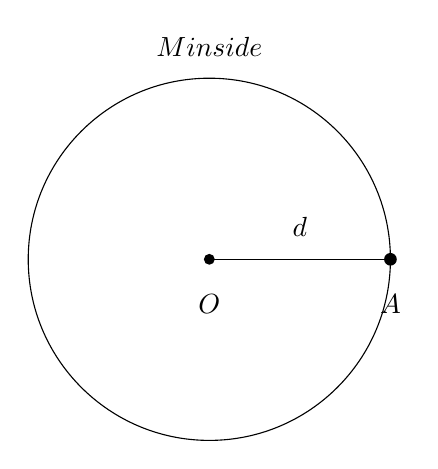
\begin{tikzpicture}[scale=1.15]
\draw (0,0) circle (2);
\fill (0,0) circle (0.06);
\fill (2,0) circle (0.07);
\draw (0,0) -- (2,0);
\draw (1,0.14) node[above] {\(d\)};
\draw (0,-0.28) node[below] {\(O\)};
\draw (2,-0.28) node[below] {\(A\)};
\draw (0,2.35) node {\(M \text{ inside}\)};
\end{tikzpicture}
\caption{Clean schematic of the Newtonian reduction: to compute the force on the representative galaxy \(A\), we keep only the mass inside the sphere of radius \(d\).}
\end{figure}

So let \(M\) be the enclosed mass. Then
\begin{equation}
M=\frac{4\pi}{3}\rho\,d^3.
\end{equation}
The galaxy's inward gravitational acceleration is therefore
\begin{equation}
-\frac{GM}{d^2}.
\end{equation}
Set this equal to the kinematical acceleration \(\ddot a\,R\):
\begin{equation}
\ddot a\,R=-\frac{GM}{d^2}.
\end{equation}
Substitute \(d=aR\) and \(M=\frac{4\pi}{3}\rho d^3\):
\begin{align}
\ddot a\,R
&=-\frac{G}{d^2}\left(\frac{4\pi}{3}\rho\,d^3\right)\nonumber\\
&=-\frac{4\pi G}{3}\rho\,d\nonumber\\
&=-\frac{4\pi G}{3}\rho\,aR.
\end{align}
Divide by \(aR\):
\begin{equation}
\frac{\ddot a}{a}=-\frac{4\pi G}{3}\rho.
\end{equation}
And substituting \(\rho=\nu/a^3\) gives the density-dilution form that also appears on the board,
\begin{equation}
\frac{\ddot a}{a}=-\frac{4\pi G\nu}{3a^3}.
\end{equation}

This is the first central dynamical equation of the lecture. It is universal. The representative radius \(R\) has dropped out, so the same equation holds for every galaxy in the homogeneous universe.

It also has an immediate consequence. If \(\rho\neq 0\), then the right-hand side is negative, so a homogeneous matter-filled universe cannot be static. Static means \(a(t)\) constant, hence \(\ddot a=0\). But \(\ddot a=0\) is possible only if \(\rho=0\). A filled homogeneous universe must evolve.

Historically the equation was discovered in the general-relativistic setting by Friedmann. The lecture's point is that, as a matter of logic, the Newtonian argument already contains the essential structure.

\subsection{Question \& Answer}

\paragraph{Question.} If every place sees matter on both sides, why is the universe not static?

\paragraph{Answer.} Because the naive symmetry argument is not the right one. It imagines that matter on one side is simply balanced by matter on the other side. Newton's theorem tells us to organize the force differently. For any chosen representative galaxy, everything outside the sphere through that galaxy gives zero net contribution, while everything inside acts as though concentrated at the center. The galaxy therefore feels an inward relative acceleration determined by the enclosed density.

The lecture also presses the point that everything hinges on homogeneity. If the mass per unit volume were not the same everywhere, then the enclosed mass would not scale universally with the volume, and the entire clean reduction to one equation for \(a(t)\) would fail.

Finally, the arbitrariness of the origin is not a defect. Had we chosen some other galaxy as the origin, the calculation would have looked different in detail, because one must transform carefully to the new frame and include the inertial terms appropriate to that motion. But the final equation would be the same. That is the only real test, and it is passed.

\section{Acceleration Is Not Velocity}

The next beat in the lecture is pedagogically crucial. We have found that
\begin{equation}
\frac{\ddot a}{a}=-\frac{4\pi G}{3}\rho.
\end{equation}
This says that the acceleration is negative. It does not yet say whether the universe is expanding or contracting. That is a statement about \(\dot a\), not \(\ddot a\).

To stop the wrong intuition before it takes hold, the lecture leaves cosmology for a moment and studies the simpler motion of a particle in the gravitational field of the Earth.

\subsection{Question \& Answer}

\paragraph{Question.} Does \(\ddot a<0\) mean that the universe is contracting?

\paragraph{Answer.} No. It means only that \(\dot a\) is being pushed downward. If \(\dot a>0\), the universe is expanding but decelerating. If \(\dot a<0\), the universe is contracting and the contraction is speeding up.

This is ordinary mechanics. A car can move forward with positive velocity while its acceleration is negative because the driver is braking. The lecture makes exactly this point in everyday language. So a negative \(\ddot a\) is not a verdict on the sign of \(\dot a\). It is only a statement that gravity is trying to slow expansion or speed contraction.

\begin{figure}[t]
\centering

\includegraphics[width=0.82\textwidth]{lecture_01_figure_04.png}
\caption{The one-particle Newtonian comparison as it appears on the board: an inverse-square force law, a radial sketch, and residual cosmology equations still visible at the left edge.}
\end{figure}

\begin{figure}[t]
\centering
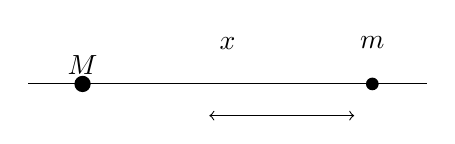
\begin{tikzpicture}[scale=1.15]
\fill (0,0) circle (0.09);
\draw (0,0) node[above] {\(M\)};
\draw (-0.6,0) -- (3.8,0);
\fill (3.2,0) circle (0.07);
\draw (3.2,0.28) node[above] {\(m\)};
\draw[->] (2.2,-0.35) -- (3.0,-0.35);
\draw[->] (2.2,-0.35) -- (1.4,-0.35);
\draw (1.6,0.45) node {\(x\)};
\end{tikzpicture}
\caption{Clean version of the one-dimensional Newtonian sketch used to separate acceleration from velocity. The source mass sits at the origin, the test particle is at distance \(x\), and the motion is along a radial line.}
\end{figure}

Let \(x\) now denote the particle's distance from the Earth. This \(x\) is not the earlier comoving coordinate. The equation of motion is
\begin{equation}
\ddot x=-\frac{GM}{x^2}.
\end{equation}
Again, the minus sign tells us only that the acceleration points inward. The particle may still be moving outward. If it is thrown upward, it has positive velocity and negative acceleration. If it is already falling inward, the same negative acceleration makes it fall faster.

So the force law alone is not enough to tell us whether the motion turns around. For that we need energy.

\begin{figure}[t]
\centering

\includegraphics[width=0.78\textwidth]{lecture_01_figure_02.png}
\caption{The beginning of the energy detour. The lecture has written the moving particle and its kinetic term, while verbally asking for the missing potential energy.}
\end{figure}

For the Earth problem the conserved energy is
\begin{equation}
E=\frac12 m v^2-\frac{GMm}{x}.
\end{equation}
This is the more useful equation for classifying the motion. If \(E<0\), the particle is bound. If \(E>0\), it has beaten escape velocity and will not come back. The edge of the parameter space is
\begin{equation}
E=0.
\end{equation}
That is the escape-velocity case. Setting \(E=0\) gives
\begin{align}
\frac12 v^2&=\frac{GM}{x},\\
v_{\mathrm{esc}}^2&=\frac{2GM}{x}.
\end{align}

Now the lecture's reason for the detour becomes clear. The expanding universe has an exact analog of these three cases: below escape velocity, above escape velocity, and exactly at the edge. The acceleration equation by itself did not distinguish them. Energy will.

\section{Zero Total Energy, Friedmann's Equation, and the \(t^{2/3}\) Law}

We now return to the representative galaxy at fixed comoving radius \(R\). For all practical purposes it knows only that it is moving in the gravitational field of a point mass \(M\) at the center. The enclosed mass stays fixed because the grid moves with the matter:
\begin{equation}
M=\frac{4\pi}{3}\rho\,a^3R^3=\frac{4\pi}{3}\nu R^3.
\end{equation}
The first equality uses the physical density and physical volume. The second uses \(\rho=\nu/a^3\). This is one of the lecture's central bookkeeping points: although the sphere grows physically as \(a(t)\) grows, the number of galaxies inside the corresponding comoving sphere does not change.

\begin{figure}[t]
\centering

\includegraphics[width=0.82\textwidth]{lecture_01_figure_05.png}
\caption{The cosmological energy formula emerging on the board. Only the numerator of the potential term is fully visible, so the denominator in the typeset formula is supplied from the transcript and the surrounding algebra.}
\end{figure}

The kinetic energy of the representative galaxy is
\begin{equation}
\frac12 m\dot a^{\,2}R^2,
\end{equation}
since its physical velocity is \(v=\dot a\,R\). Its potential energy is
\begin{equation}
-\frac{GMm}{aR}.
\end{equation}
Therefore
\begin{equation}
E=\frac12 m\dot a^{\,2}R^2-\frac{GMm}{aR}.
\end{equation}

The lecture now chooses the simplest case: the total energy is exactly zero. This is the cosmological analog of exactly escape velocity.
\begin{equation}
E=0.
\end{equation}
Cancel the test mass \(m\), multiply by \(2\), and divide by \(a^2R^2\):
\begin{align}
0&=\frac12 \dot a^{\,2}R^2-\frac{GM}{aR},\\
\left(\frac{\dot a}{a}\right)^2&=\frac{2GM}{a^3R^3}.
\end{align}
Now introduce the physical volume of the sphere,
\begin{equation}
V=\frac{4\pi}{3}a^3R^3,
\end{equation}
and write
\begin{equation}
\frac{M}{V}=\rho.
\end{equation}
Then
\begin{equation}
\left(\frac{\dot a}{a}\right)^2=\frac{8\pi G}{3}\rho.
\end{equation}
This is the Friedmann equation in the zero-energy matter-only case.

The lecture stresses that this is the form usually written, and that it is equivalent to the earlier acceleration equation for the special case at hand just as energy conservation and Newton's second law are equivalent for an ordinary particle.

Substituting the earlier density relation gives
\begin{equation}
\left(\frac{\dot a}{a}\right)^2=\frac{8\pi G\nu}{3a^3}.
\end{equation}
Since \(\nu\) is merely the mass per unit coordinate volume, its numerical normalization depends partly on the choice of coordinates. The lecture therefore strips the equation down to its essential form by absorbing the constant:
\begin{equation}
\left(\frac{\dot a}{a}\right)^2=\frac{1}{a^3}.
\end{equation}
This is the matter-dominated Newtonian universe with no cosmological constant. It is the standard decelerating model that dominated the subject before late-time acceleration was discovered.

\begin{figure}[t]
\centering

\includegraphics[width=0.74\textwidth]{lecture_01_figure_06.png}
\caption{Matter-dominated Friedmann scaling on the board, first with constants and then in normalized form. This is the algebraic basis for the statement that the expansion slows but never reaches a turnaround in the zero-energy case.}
\end{figure}

There is a qualitative conclusion before we solve anything. The right-hand side is always positive for finite \(a\). Therefore \(H^2=(\dot a/a)^2\) never reaches zero. But a turnaround would require \(\dot a=0\). So in the zero-energy case the expansion slows forever without ever stopping. The lecture's phrase is memorable: the universe gets tired of expanding, but never tired enough to stop.

To solve the equation, the lecture takes the easy route and tries a power law:
\begin{equation}
a(t)=Ct^p.
\end{equation}
Then
\begin{align}
\dot a&=Cp\,t^{p-1},\\
\frac{\dot a}{a}&=\frac{p}{t},\\
\frac{1}{a^3}&=\frac{1}{C^3 t^{3p}}.
\end{align}
Substitute into the normalized Friedmann equation:
\begin{equation}
\frac{p^2}{t^2}=\frac{1}{C^3 t^{3p}}.
\end{equation}
Matching the powers of \(t\) gives
\begin{equation}
3p=2,
\end{equation}
hence
\begin{equation}
p=\frac23.
\end{equation}
Matching the coefficients then fixes the constant \(C\) in the chosen normalization, but the lecture emphasizes that the exponent is the important part. We conclude that
\begin{equation}
a(t)\propto t^{2/3}.
\end{equation}

That is the expansion law of the Newtonian matter-dominated universe at the critical escape velocity. It is also the point where the lecture pauses and admires the result. Newton, in principle, could have gotten this far.

The story is not finished. If the total energy is not zero, another term appears. As a cautious preview, the next step takes the form
\begin{equation}
\left(\frac{\dot a}{a}\right)^2=\frac{8\pi G}{3}\rho+\frac{C}{a^2},
\end{equation}
where this \(C\) remembers the total energy and is unrelated to the amplitude \(C\) in the trial solution above. If \(C>0\), the universe has beaten escape velocity. If \(C<0\), it will eventually re-collapse.

And then comes the modern correction. The real universe does not continue curving downward forever. It begins that way, but later curves upward. So the model derived in this lecture is both real and incomplete: real because it captures the matter-dominated Newtonian physics cleanly, incomplete because the actual universe contains an additional ingredient that causes acceleration.

\section{Summary}

The lecture unfolds in a strict order, and that order is part of the physics. We begin with isotropy, use it to motivate homogeneity, and adopt the cosmological principle as a large-scale averaged description. We then choose comoving coordinates so that galaxies are frozen into an expanding grid. From that alone, the scale factor \(a(t)\) and Hubble's law appear as kinematics.

Only then does Newton enter. Newton's theorem reduces the many-body problem to the enclosed mass inside a sphere, and that gives the universal acceleration equation
\begin{equation}
\frac{\ddot a}{a}=-\frac{4\pi G}{3}\rho.
\end{equation}
The Earth-projectile analogy then clarifies the sign of this equation: negative acceleration is not the same thing as negative velocity.

Finally, energy conservation supplies what the force law could not. In the zero-energy case we obtain the matter-dominated Friedmann equation
\begin{equation}
\left(\frac{\dot a}{a}\right)^2=\frac{8\pi G}{3}\rho,
\end{equation}
and with \(\rho=\nu/a^3\) this leads to
\begin{equation}
a(t)\propto t^{2/3}.
\end{equation}
So the first lecture arrives at a full model universe: homogeneous, matter-dominated, Newtonian, decelerating, and exactly at the threshold between eternal expansion and eventual collapse. The next step is to move away from zero total energy, and then beyond that to the real accelerating universe.